
\medskip

On considère la fenêtre de téléchargement ci-dessous.
\begin{center}
	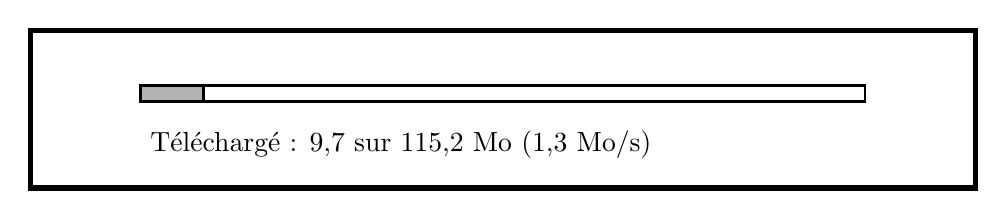
\begin{tikzpicture}[]
		\draw[line width = 2pt] (0,0) rectangle (12,2);
		\draw [line width = 1pt, fill = gray!60]  (1.4,1.1) rectangle (2.2,1.3);
		\draw [line width = 1pt]  (1.4,1.1) rectangle (10.6,1.3);
		\node [right] at (1.4,0.55) {Téléchargé : 9,7 sur 115,2 Mo (1,3 Mo/s)};
	\end{tikzpicture}
\end{center}

Si la vitesse de téléchargement reste constante, faudra-t-il plus d'une minute et vingt-cinq secondes pour que le téléchargement se termine ?
